Here I decompose the four series of the aggregate labour share using both the shift-share and Haltiwanger methods for the industry-level data. 


% In figures \ref{fig:decomp_1}, \ref{fig:decomp_2to3} and \ref{fig:decomp_4}, I plot the cumulative path of the Between, Within, and Cross terms estimated for each year. 

\subsection{Payroll Labour Share}
I begin by decomposing the payroll labour share. The advantage of examining the payroll labour share is that payroll labour income represents the part of the labour share accruing unambiguously to labour. Figure \ref{fig:decomp_1} shows the cumulative paths of the between, within, and cross terms estimated for each year using both the shift-share and Haltiwanger decomposition. 

The left panel in figure \ref{fig:decomp_1} shows the cumulative between-sector terms for each decomposition. The shift-share decomposition replicates the results from \citet{elsbyDeclineLaborShare2013a} and estimates that between-sector reallocation adds a cumulative -0.1pp to the labour share from 1987 to 2011, around 4\% of the total decline. Using the shift-share decomposition, one would conclude there is a zero reallocation effect. However, the cross effect estimated in the Haltiwanger decomposition is negative and growing over time. Via Theorem \ref{theorem_1}, a negative cross term reduces the shift-share between-sector term relative to the Haltiwanger between-sector term. The Haltiwanger decomposition estimates that reallocation cumulatively adds 1.7pp to the payroll labour share, around -47\% of the total decline. The Haltiwanger decomposition recovers a positive reallocation effect, in line with the counterfactual evidence presented in Section \ref{sec:puzzle} and in contrast to previous studies. 

Moreover, the negative within-sector contribution in the shift-share decomposition is overestimated due to the negative cross term. In the right panel, The shift-share decomposition apportions 96\% of the total decline in the labour share to within-sector mechanisms, whereas the Haltiwanger decomposition apportions only 45\%. Since the between, within, and cross contributions add up to 100\%, the Haltiwanger decomposition implies co-movements between sectoral weights and labour shares account for 102\% of the decline in the labour share. The negative co-movement between $\omega_{it}$ and $\lambda_{it}$ is the dominant factor in the declining payroll labour share. 

% * and then do the variance decomposition with respect to wl and va (have to use price indexes??)


\begin{figure}[h]
  \centering
\caption{\normalsize Cumulative decomposition of the payroll labour share}
\subfloat[Between-sector contributions]{\label{fig:elsby_hw}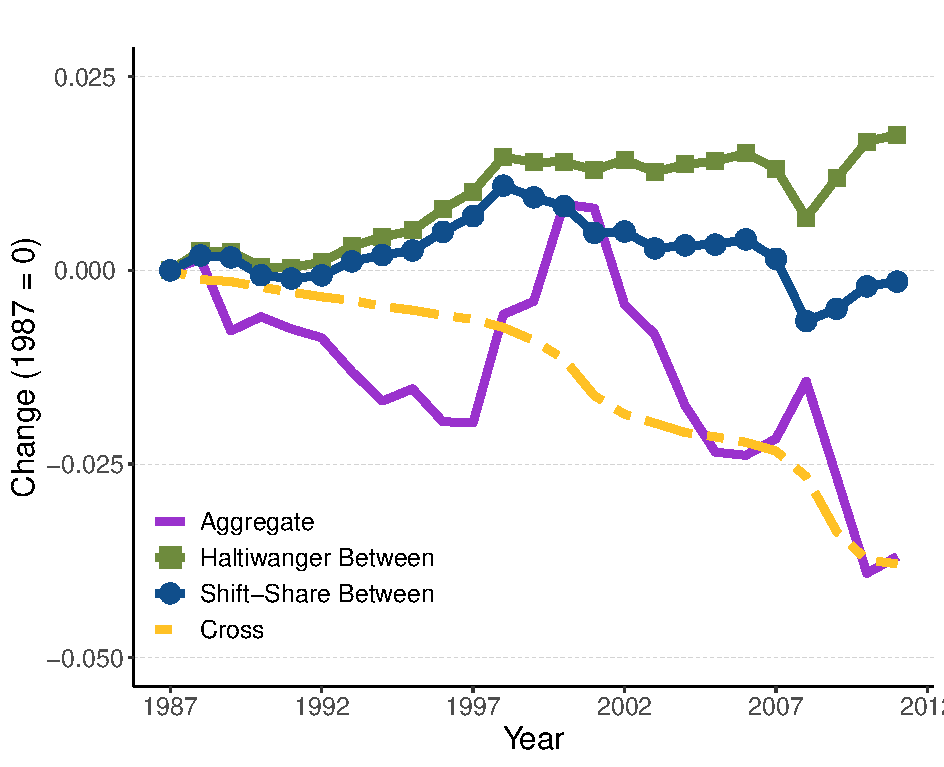
\includegraphics[width=.45\linewidth]{Decomposition/elsby_Between_D_graph.pdf}}
\subfloat[Within-sector contributions]{\label{fig:elsby_hw}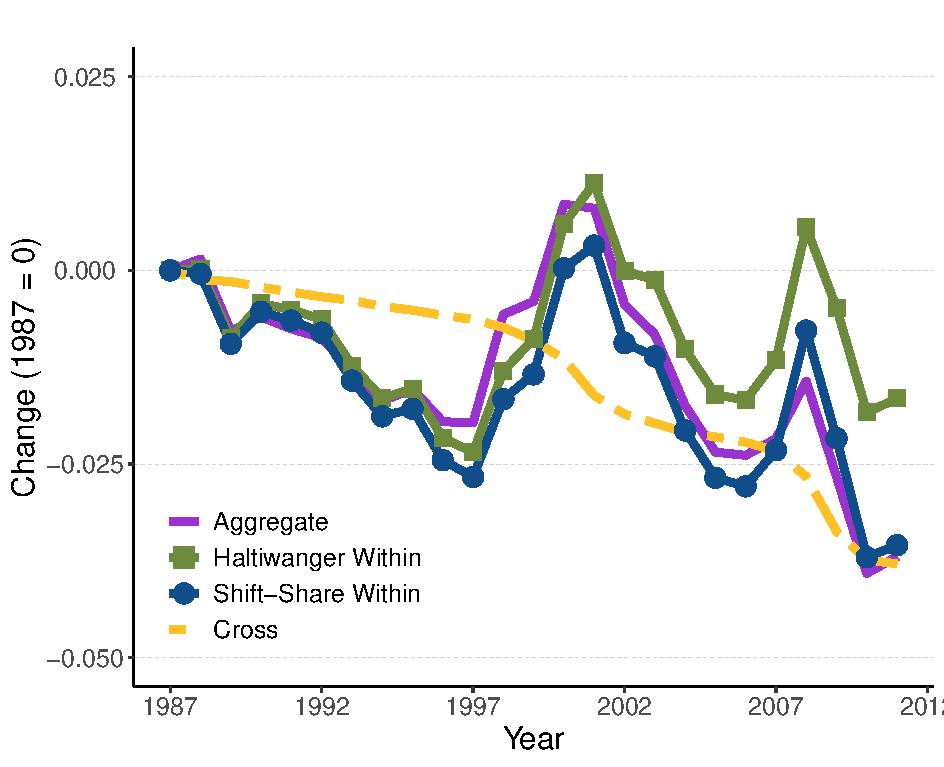
\includegraphics[width=.45\linewidth]{Decomposition/elsby_Within_D_graph.pdf}}\vfill
\begin{minipage}{\linewidth}
    \caption*{\textit{Notes}: Cumulative between, within and cross terms for both decomposition methods using the `payroll labour share' approach, 1987 to 2011. `0.05' on the y-axis corresponds to 5 percentage points (pp). The Aggregate and Cross lines are equivalent across both panels. \\
    \textit{Source}: BEA, \citet{elsbyDeclineLaborShare2013a} replication package, and author's calculations.}
\end{minipage}
\label{fig:decomp_1}
\end{figure}

The Haltiwanger cross term is negative since changes in value-added affect sectoral weights and sectoral labour shares in opposite directions: $VA_{it}$ appears in the numerator and denominator, respectively. Appendix \ref{sec: veil} shows the cross term is negative for virtually every sector analysed. 
% Furthermore, Appendix \ref{} demonstrates the variance in sectoral labour shares in each year is largely accounted for by the covariance between sectoral labour income $WL_{it}$ and sectoral value-added $VA_{it}$, rather than the variance of $WL_{it}$ or $VA_{it}$ by itself. 
Given the quantitative importance of the cross term, my results imply value-added dynamics within sectors are important for the path of the aggregate payroll labour share. \citet{kehrigMicroLevelAnatomyLabor2021a} report a similar finding using establishment-level data in the US manufacturing sector. 


\subsection{Accounting For Self-Employed Labour Income}

While the payroll labour share captures the part of the aggregate labour share accruing unambiguously to labour income, how do the results differ when self-employed labour income is accounted for? Figures \ref{fig:decomp_2}, \ref{fig:decomp_3}, and \ref{fig:decomp_4} plot the cumulative shift-share and Haltiwanger decompositions for the three self-employed labour income imputation methods I use. In contrast to the `payroll labour share' results, all three shift-share decompositions estimate a positive and non-negligible reallocation effect. Looking at the three left panels in figures \ref{fig:decomp_2}, \ref{fig:decomp_3}, and \ref{fig:decomp_4}, between-sector changes add to the aggregate labour share measures. Nevertheless, each panel shows the cross effect is negative, so, as a result, the shift-share decomposition undercounts the positive reallocation effect and overcounts the negative within-sector effect. Netting out the impact of the co-movement, the Haltiwanger decomposition lines show that reallocation adds between 14.5pp and 27.7pp more to the aggregate labour share than the shift-share method estimates. Similarly, the Haltiwanger decomposition estimates that declining labour shares within sectors account for between 14.5pp and 27.7pp less than the shift-share method estimates. 

Table \ref{tab:rr} indicates the number of percentage points that the shift-share decomposition undercounts the effect of reallocation and overcounts the effect of declining labour shares within sectors relative to the Haltiwanger decomposition. Regardless of the labour share definition, using the shift-share method severely undercounts the positive effect of reallocation and loads onto the within-sector contribution. From the cumulative Haltiwanger decompositions in figures \ref{fig:decomp_1}, \ref{fig:decomp_2}, \ref{fig:decomp_3}, and \ref{fig:decomp_4}, the quantitative importance of all three channels - between, within, and cross - for changes in the aggregate labour share emerges. Sectoral labour shares cannot be studied in isolation to examine the decline of the aggregate labour share. 

% The large and negative cross term for each labour share variation leads to a positive between-sector term being undercounted and a negative within-sector term being overcounted when using the shift-share decomposition. In Table \ref{tab:rr} I indicate by how many percentage points the under- and overcounting occurs. Depending on the definition of the labour share used, the shift-share decomposition undercounts a positive between-sector term by between 14.5 and 51.3 percentage points. Since Theorem \ref{theorem_1} shows the cross term is split evenly across the shift-share between- and within-sector terms, the negative within-sector contribution is overcounted by between 14.5 and 51.3 percentage points. Regardless of the labour share definition used, there is considerable under- and overcouting occurring. 



{\setstretch{1.0}

\begin{figure}[h]
  \centering
\caption{\normalsize Cumulative decompositions of aggregate labour share}
\subfloat[Between-sector]{\label{fig:klems_hw}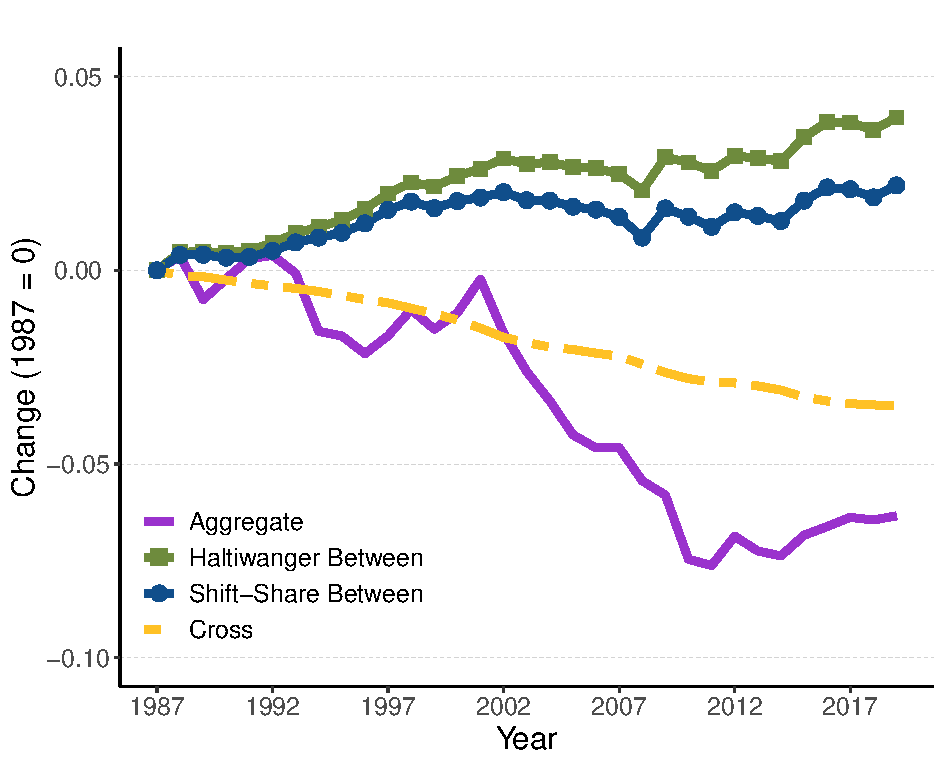
\includegraphics[width=.45\linewidth]{Decomposition/Between_D_graph.pdf}}
\subfloat[Within-sector]{\label{fig:klems_hw}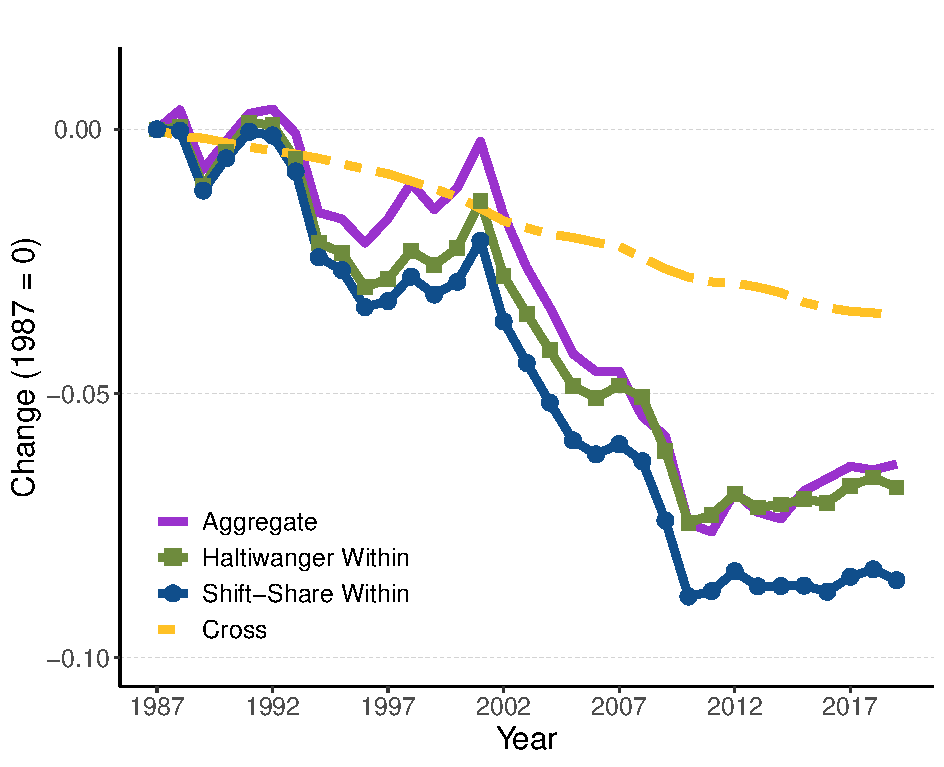
\includegraphics[width=.45\linewidth]{Decomposition/Within_D_graph.pdf}}\vfill
\begin{minipage}{\linewidth}
    \caption*{\textit{Notes}: Cumulative between, within and cross terms for both decomposition methods using the `same-wage-distribution' assumption, 1987-2019. `0.05' on the y-axis corresponds to 5 percentage points (pp). The scale of the left and right panels are different, but the Aggregate and Cross lines are equivalent. \\
    \textit{Source}: BEA-BLS integrated industry-level production account and author's calculations.}
\end{minipage}
\label{fig:decomp_2}
\end{figure}
}

\begin{figure}[h]
  \centering
\caption{\normalsize Cumulative decompositions of aggregate labour share}
\subfloat[Between-sector]{\label{fig:mm_ss}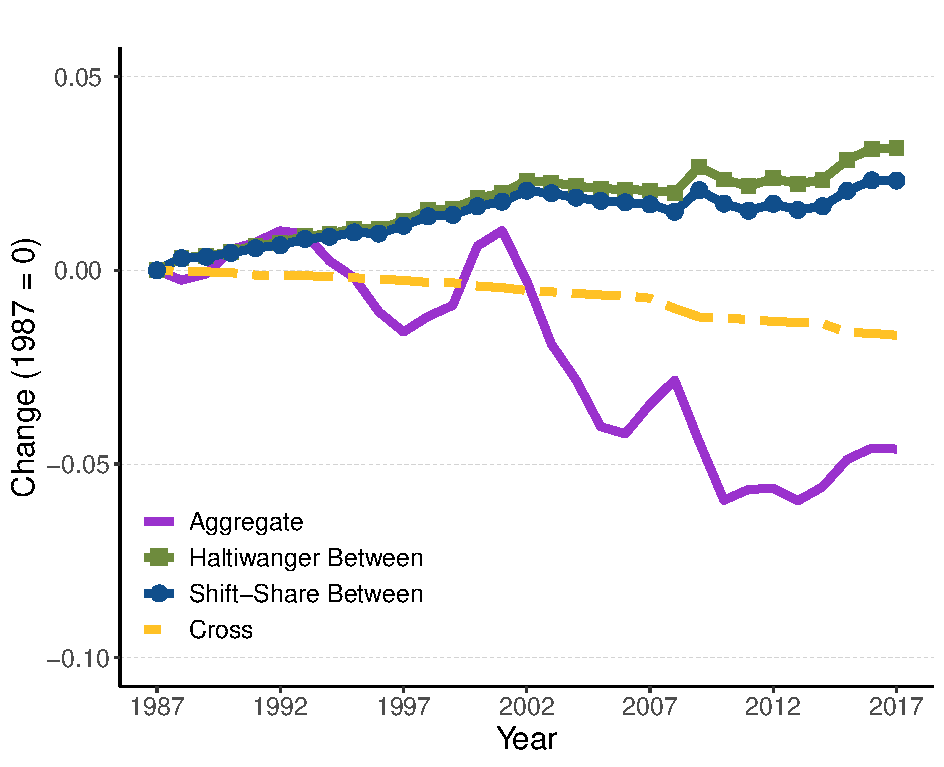
\includegraphics[width=.45\linewidth]{Decomposition/mm_Between_D_graph.pdf}}
\subfloat[Within-sector]{\label{fig:mm_hw}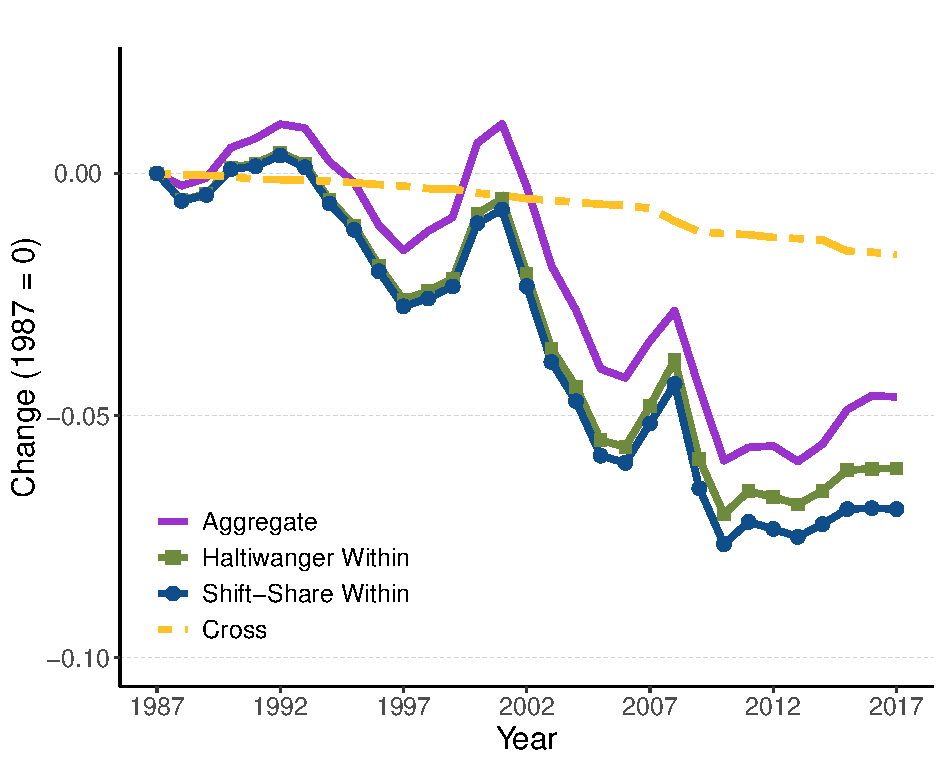
\includegraphics[width=.45\linewidth]{Decomposition/mm_Within_D_graph.pdf}}\vfill
\begin{minipage}{\linewidth}
    \caption*{\textit{Notes}: Cumulative between, within and cross terms for both decomposition methods using the `same-labour-share' assumption, 1987-2017. `0.05' on the y-axis corresponds to 5 percentage points (pp). The scale of the left and right panels are different, but the Aggregate and Cross lines are equivalent. \\
    \textit{Source}: BEA, BLS, \citet{mendieta-munozDeclineUSLabor2021} replication package, and author's calculations.}
\end{minipage}
\label{fig:decomp_3}
\end{figure}

\begin{figure}[h]
  \centering
\caption{\normalsize Cumulative decompositions of aggregate labour share}
\subfloat[Between-sector]{\label{fig:ew_ss}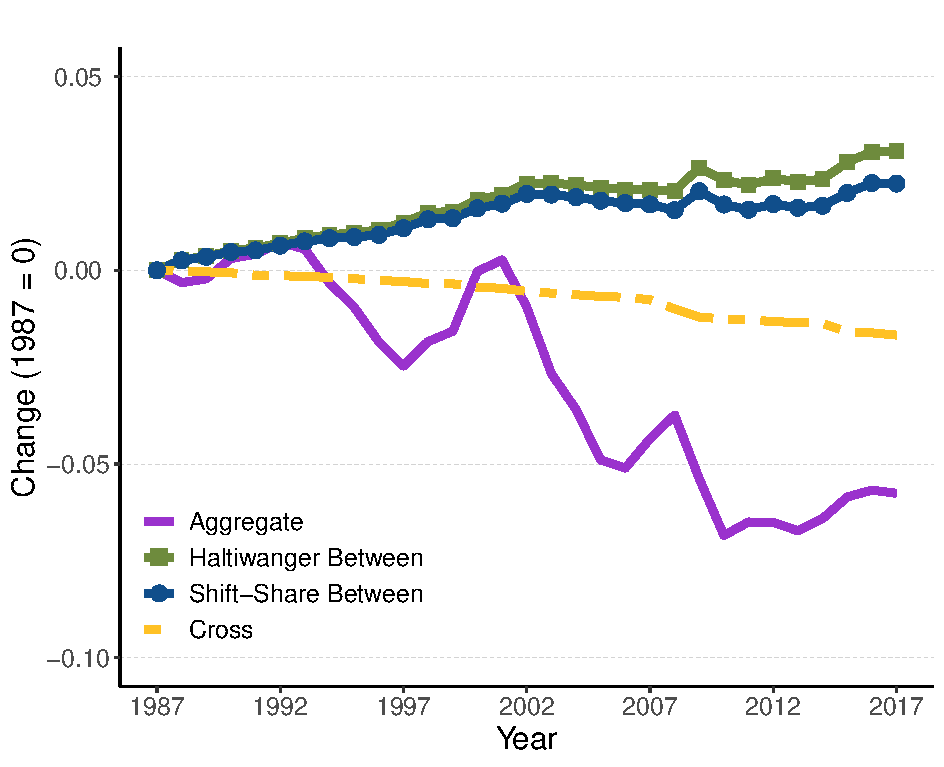
\includegraphics[width=.45\linewidth]{Decomposition/ew_Between_D_graph.pdf}}
\subfloat[Within-sector]{\label{fig:ew_hw}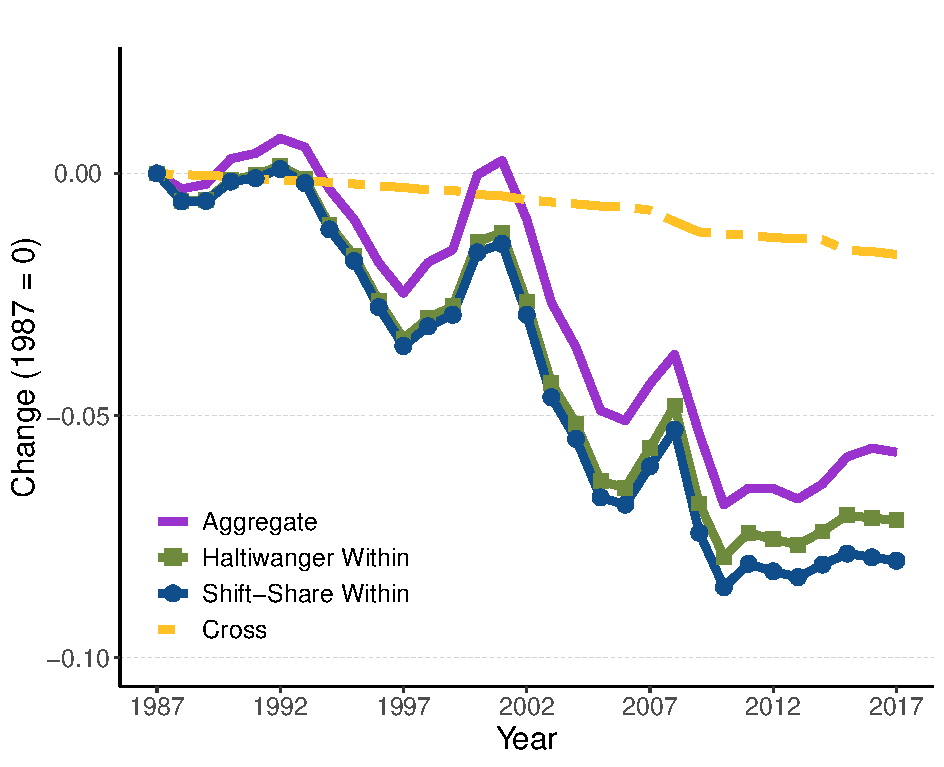
\includegraphics[width=.45\linewidth]{Decomposition/ew_Within_D_graph.pdf}}\vfill
\begin{minipage}{\linewidth}
    \caption*{\textit{Notes}: Cumulative between, within and cross terms for both decomposition methods using the `economy-wide labour share' assumption, 1987-2017. `0.05' on the y-axis corresponds to 5 percentage points (pp). The scale of the left and right panels are different, but the Aggregate and Cross lines are equivalent. \\
    \textit{Source}: BEA, BLS, \citet{mendieta-munozDeclineUSLabor2021} replication package, and author's calculations.}
\end{minipage}
\label{fig:decomp_4}
\end{figure}


\begin{table}[h]
    \centering
    \small
    \caption{\normalsize Percentage point under- or over-counting of shift-share relative to Haltiwanger decomposition}
    \begin{tabular}{lcc}
       \toprule[1.1pt]
        
        & Between-sector undercounted & Within-sector overcounted \\
        
        \cmidrule[0.8pt](lr{0.125em}){2-3}

       \textbf{A. Payroll labour share.} & \multirow{2}{*}{-51.3} & \multirow{2}{*}{51.3} \\
       \textit{Years}: 1987-2011 &  &  \\

       \textbf{B. Same-wage-distribution.} & \multirow{2}{*}{-27.7} & \multirow{2}{*}{27.7}\\
       \textit{Years}: 1987-2019 &  &  \\

       \textbf{C. Same-labour-share.} & \multirow{2}{*}{-18.2} & \multirow{2}{*}{18.2}\\
       \textit{Years}: 1987-2017 &  &  \\

       \textbf{D. Economy-wide.} & \multirow{2}{*}{-14.5} & \multirow{2}{*}{14.5}  \\
       \textit{Years}: 1987-2017 &  &  \\       
       \bottomrule[1.1pt]
    \end{tabular}
    
\begin{minipage}{\linewidth}
\captionsetup{justification=raggedright,singlelinecheck=false}
    \caption*{\textit{Notes}: The `Between-sector undercounted' column subtracts the percentage of the labour share decline accounted for by the shift-share between-sector term from the percentage accounted for by the Haltiwanger between term. The `Within-sector overcounted' column subtracts the shift-share within-sector term from the Haltiwanger within-sector term. I calculate the amount for each labour share definition and sample period. \\
    \textit{Source}: BEA, BLS, and author's calculations.}
\end{minipage}
    \label{tab:rr}
\end{table}


% Lastly, to get a numerical idea of how much of the total change in the labour share is accounted for by reallocation, I divide the cumulative between-effect by the decline in the aggregate labour share (the endpoints of the Between and Aggregate lines in figures \ref{fig:decomp_1}, \ref{fig:decomp_2to3} and \ref{fig:decomp_4}). Both ``Between/ Total'' columns in Table \ref{tab:rr} show the Haltiwanger between-sector effect accounts for over one-third of the total change in the labour share, regardless of the labour share definition and years examined. 

% \begin{table}[h]
%     \centering
%     \small
%     \begin{tabular}{lcc cc}
%        \toprule[1.1pt]
%         & \multicolumn{2}{c}{1987-2011} & \multicolumn{2}{c}{} \\
        
%         \cmidrule[0.8pt](lr{0.125em}){2-3}
%         \cmidrule[0.8pt](lr{0.125em}){4-5}
        
%         & $\Delta$ labour share & Between/ Total & $\Delta$ labour share &  Between/ Total \\
        
%         \cmidrule[0.8pt](lr{0.125em}){1-1}
%         \cmidrule[0.8pt](lr{0.125em}){2-3}
%         \cmidrule[0.8pt](lr{0.125em}){4-5}
        
%        \textbf{A. Same-wage-distribution.} &  &  & \multicolumn{2}{c}{1987-2019} \\
%        \cmidrule[0.8pt](lr{0.125em}){4-5}
%        Haltiwanger & -7.6pp & -33.6\% & -6.3pp & -62.3\%\\
%        Shift-Share & -7.6pp & -14.7\% & -6.3pp & -34.6\%  \\
%        \textbf{B. Same labour share.} &  &  & \multicolumn{2}{c}{1987-2017} \\
%        \cmidrule[0.8pt](lr{0.125em}){4-5}
%        Haltiwanger & -5.7pp & -38.4\% & -4.6pp & -68.4\% \\
%        Shift-Share & -5.7pp & -27.2\% & -4.6pp & -50.2\% \\
%        \textbf{C. Economy-wide.} &  &  & \multicolumn{2}{c}{1987-2017} \\
%        \cmidrule[0.8pt](lr{0.125em}){4-5}
%        Haltiwanger & -6.5pp & -33.8\% & -5.8pp & -53.5\% \\
%        Shift-Share & -6.5pp & -24.1\% & -5.8pp & -39.0\% \\
%        \textbf{D. Payroll labour share.} &  &  &  &  \\
%        Haltiwanger & -3.7pp & -47.3\% & - & - \\
%        Shift-Share & -3.7pp & 4.0\% & - & - \\
%        \bottomrule[1.1pt]
%     \end{tabular}
%     \caption{The first and third data columns show the total change in the labour share for the years 1987 to 2011 and then for 1987 to the final year in each labour share definition sample. The ``Between/ Total'' column divides the cumulative between-sector effect for the Haltiwanger and shift-share decompositions by the total change in the labour share. I leave a discussion to Appendix \ref{sec: reallocation_payroll} examining why the shift-share reallocation ratio is only zero when the payroll labour share is used.}
%     \label{tab:rr}
% \end{table}





